\maketitle
%\thispagestyle{fancy}
\section*{Overview}

\subsection*{Goals}

Our goals for this month were as follows: 

\begin{itemize}
  \item 
    Identify concrete objective functions for the Swarm incentive system with a view to multi-objective optimisation.
  \item
    Study the convergence of system state on allocatively efficient equilibria.
  \item
    Inspect historic activity in the Swarm stake registry and look for evidence of competitive behaviour.
\end{itemize}

\subsection*{Methodology}

We used a classical microeconomic equilibrium approach to formulating abstract objectives for the Swarm economy, then mechanism design to interpret the supply function in terms of the actual redistribution game.

For studying activity on the stake registry, we pulled historic log data from the stake registry contract, matched block numbers with known significant network events to pick suitable date ranges, and built a Python notebook to calculate basic statistics and create visualisations.\footnote{\url{https://github.com/shtukaresearch/swarm-staking/blob/main/marimonb/swarm-data.py}}

\subsection*{Scope}

We formulated the objectives using a minimal supply-and-demand model for Swarm storage where the details of the redistribution mechanism is abstracted away.
%
For evaluating a specific iteration of Swarm against these objectives, we used the storage incentive system deployed between versions 0.6.0 and 0.9.1.\footnote{The changes introduced in the new Redistribution contract deployed in v0.8.6 are out of scope for our model.}

The observational study focused on the version of the stake registry bundled with v0.4.0 of the storage incentive system (deployed block 25,527,075) and deprecated with v0.9.1 (block 35,961,749).
%
For more details, see \textbf{Findings}.

\section*{Operations management}

\subsection*{Completed Milestones}

\begin{itemize}
  \item 
    Expand on candidate list of quantitative objectives for the Swarm staking system.
  \item 
    Develop stochastic perfect information model that captures core aspects of the current staking system. 
    %
    Use solutions to the deterministic model to back out results that hold in expectation.

  \item Study staker decision processes and risks without the assumptions of determinism.
  
  \item Establish conditions for market clearing at the target replication rate.
  
  \item Identify aggregate economic indicators and metrics relevant for monitoring and forecasting Swarm storage performance and making decisions about improvements.

  
  \item Pull data on historic staker behaviour and analyse it in the context of our model. Are there any stakers that already exhibit strategic behaviour? How frequent are instances of direct competition in acquiring stake positions? Create visualisations.
\end{itemize}

\subsection*{Future milestones}

\begin{itemize}
  \item Compile formal report and executive summary.
\end{itemize}

\subsection*{Revised milestones}

\begin{itemize}
  \item Numerical solution of Bellman equation for $n$-step strategies in the stochastic setting. 
  
  In the September report, it was claimed that optimal $n$-step policies terminate in one step under perfect information and stationarity.
  %
  This is not true.
  %
  However, due to time constraints we propose to defer numerical estimation of these policies to a future project.

  
  \item Study staker decision processes without the assumptions of complete information or stationarity. Due to time constraints, this will have to be left to a future project.

\end{itemize}


\subsection*{Schedule}

\paragraph{November} Compile formal LaTeX report. Gather recommendations and compose roadmap for future research.

\paragraph{December} \emph{fin}



\section*{Findings}

\subsection*{Summary}

\begin{itemize}
  \item We established that a formal notion of allocative efficiency of equilibria is needed for lower operating costs to be passed on to users as lower prices. We related this efficiency objective to a basic objective of maximising demand.
  \item The current implementation of Swarm network allows neighbourhoods to reach a state from which an allocatively efficient equilibrium can never be reached, given that new NOs with lower costs enter the game.
  %
  In order to address this problem, new ways for stake to be reallocated --- either by trading or liquidation --- should be introduced.
  \item We retrieved \code{StakeUpdated} events, grouped them together into 10 bit neighbourhoods, and searched for an appropriately defined notion of `competitive' behaviour.
  %
  While we did observe activity that could be evidence of competition, in all cases there were also other plausible explanations, such as the split into 11 bit neighbourhoods.
\end{itemize}

\subsection*{Price optimisation}

We revised and clarified our approach to defining system design objectives, identifying specific objective functions and studying their implementation through a mechanism design approach.

The key objective functions under study this month were the dual optimisation problems:
\begin{enumerate}
  \item Minimise storage price subject to QoS constraints;
  \item Maximise QoS at a given price.
\end{enumerate}
%
We evaluate QoS purely in terms of replication rate.
%
The design of the Swarm protocol calls for this to have a target value of $4$; but presumably, if a strictly higher replication rate can be provided for the same or lower price, this would also be fine.
%
Note that if the Swarm storage service is an ordinary good, objective (1) is equivalent to maximisation of the quantity demanded subject to the QoS constraint.

\paragraph{Production model}
Let us fix a demand quantity $D>0$ and allow excess supply to be absorbed as higher replication rate.
%
If we write $\mathcal{P}=\uR$ for price space, and $\mathcal{Q}=\uR$ for QoS (replication rate) space, then the Swarm protocol rules and exogenous world state determines a set of \emph{feasible production profiles}
%
\[
  X \subset \mathcal{P}\times\mathcal{Q}
\]
%
for each quantity $D$.
%
A point $(p,q)$ is feasible if the network revenue $R=pD$ can be distributed among a population of storage providers \emph{in some way} such that they would collectively be prepared to meet the demand $D$ with replication rate $q$, i.e.~provide $qD$ units of storage.
%
The means by which this distribution is achieved is within the purview of the Swarm protocol designers.

The price optimisation problem is to find the feasible production profile $(p^*,q)$ with minimal $p$ given $q$.
%
To transform this into the dual problem of optimising $q$ given $p$, look for a selection rule 
\[
  q^*:\mathcal{P}\rightarrow X\cup\{\bot\}
\]
that assigns a feasible production profile $q^*(p)=(p,q^*)\in X\cap (\{p\}\times\mathcal{Q})$ that maximises $q^*$.
%
By the law of supply, $q^*(p)$ is increasing in $p$.\footnote{See (Mas-Collel, 1995), Chapter 5.}
%
It follows that a Pareto efficient, price-minimising production profile is obtained by finding the minimal $p$ such that $q^*(p)\geq 4$.

\paragraph{Redistribution mechanisms}
Whether or not a price-optimal feasible production profile is actually implementable depends on the details of how revenue $pD$ is redistributed among storage providers and their individual production costs.
%
That is, it depends on the choice of a budget-balanced redistribution \emph{mechanism}
\[
  \mathbf{M}:\uR \times \State \rightarrow \uR^\Overlay,
\]
that determines the amount $r_a=\mathbf{M}(R,\xi)_a$ each address $a\in\Overlay$ receives based on the total revenue $R\in\uR$ and some internal state vector $\xi\in\State$ that controls the redistribution, together with a (Bayes-Nash) equilibrium $\xi^*(R)\in\State$.

The internal state space $\State$ can take several forms, but we ask that it at least record whether each node is \emph{active} via a map $\mathtt{state}:\State\times\Overlay\rightarrow \{\mathtt{off},\mathtt{on}\}$.
%
Then we can define the \emph{replication rate} of the equilibrium $\xi^*$ by the formula
\[
  q(\xi^*) = \#\{a\in\Overlay \mid \mathtt{state}(\xi^*,a)=\mathtt{on}\}.
\]
In this case, we say that $(\mathbf{M},\xi^*)$ \emph{implements} $q$.
%
We want to find redistribution mechanisms $(\mathbf{M},\xi^*)$ that implement $q^*(p)$, or as close to it as possible, for each price $p$.

\begin{example*}In the version of the Swarm mechanism under consideration, the endogenous state vector $\xi^*$ consists of a mapping $(\mathtt{state},x):\Overlay\rightarrow \{\mathtt{off},\mathtt{on}\}\times\uR$ that identifies whether a node is active and what their equity balance is.
\end{example*}

\paragraph{Identifying an optimal allocation}
Suppose we have access to the variable costs $O:\Overlay\rightarrow\uR$ of each NO, that is, the cost of providing a single active node.
%
For simplicity, we assume that $O$ does not depend on the quantity of storage provided.\footnote{This is not as ridiculous as it sounds if we assume that NOs must reserve a certain amount of computation to run their node, regardless of how full the reserve is, and that realised demand does not stray past a power of two, triggering a neighbourhood split.}
%
Assume also that $\Overlay=\{0,\ldots,N\}$ is integer indexed and that $O(a)$ is increasing in $a$, i.e.~the node addresses are sorted in order of increasing operating cost.

It is not hard to show that it is QoS-optimal to allocate revenue share to the $K$ nodes with the lowest costs, where $K$ is chosen as large as possible.
%
\begin{proposition*}
  Under the above assumptions, let $K\in\Overlay$ be the maximum index such that
  \[
    \sum_{k=0}^KO(k) \leq R.
  \]
  Then the redistribution weights
  \[
    w_k = \left\{ \begin{array}{ll}
      O(k)/\sum_{i=0}^KO(i) & k\leq K \\
      0 & k > K
    \end{array} \right.
  \]
  define a QoS-optimal allocation with replication rate $K$.
\end{proposition*}

The Swarm protocol does not have direct access to the quantities $O(a)$, so the preceding mechanism cannot be implemented as stated.
%
Instead, we must rely on the laws of competition to induce rellocation of market share to the NOs with lowest costs.

\paragraph{Does the Swarm redistribution mechanism implement $(p^*(4),4)$?}

Due to the phenomenon of investment saturation we identified in August --- where stake positions become dilute enough that any newly issued share is worth less than its price --- there are plausible initial conditions where all issued shares end up permanently associated with a single entity.
%
In other words, no matter how much lower are the costs of prospective new entrants than the incumbent, there is no incentive-compatible way for equity to be transferred to the new entrants and hence achieve a QoS-optimal allocation.

\begin{proposition*}
  Let $i$ be an NO with cost $O_i$. 
  %
  Suppose that $i$ has an exclusive first-move opportunity to acquire shares in an as-yet unoccupied neighbourhood.
  %
  For all sufficiently low cost-revenue ratios $O_i/R$, there exists a position $s$ that $i$ may acquire such that:
  \begin{enumerate}
    \item for all NO populations $O:\Overlay\rightarrow\uR$, there is a time-invariant Nash equilibrium in which no new stake updates are made and $i$ remains the sole stakeholder;
    \item It is individually rational for $i$ to make the initial investment $s$; i.e.~$i$ earns at least $s$ in total discounted future profit from his investment.
  \end{enumerate}
  Moreover, $O_i/R\leq \frac{3-\sqrt{5}}{2}> 0.32$ is sufficiently low.
\end{proposition*}

It follows that the Swarm redistribution mechanism does not reliably implement $(p^*(q),q)$ for any $q>1$.
%
What can we do to address this problem?

\paragraph{Unlocking efficient allocations with free trade}
If we posit a market in which stake positions can be freely traded at any price, then unsurprisingly we find that the feasible trades generally result in transfers of stake from NOs with higher costs to those with lower costs, improving efficiency.
%
Thus in order for Swarm's equity allocation to reliably reach QoS-optimal equilibria, it is sufficient to allow stake positions to be transferred and traded under arbitrary market structures.
%
However, this is not the only way to achieve this: for example, it is also sufficient to allow stake to be liquidated so that it may then be reissued to another party with a higher valuation for the position.

\subsection*{Observational studies}

To establish whether any NOs are already behaving competitively, we gathered logs associated to \code{StakeUpdated} events emitted by the Stake Registry contract, grouped them into bins by overlay address prefix, and searched for examples of `reactive' update behaviour.

\paragraph{Observation period}
We drew observations from the deployment of v0.4.0 of the stake registry contract in block 25,527,075 until its pausing in block 35,963,617.\footnote{It might make sense to cut things off at the slightly earlier time of block 35,961,749, when version 0.9.1 of the stake registry contract incorporating rules from SWIP-19 and SWIP-20 was deployed, but since the difference was just 2 hours and 20 minutes, we ignore this.} This represents about 2 years of network activity.

We noticed substantial staking activity among new overlay addresses in October and November of 2023, presumably an impact of the thousands of new active nodes that reportedly appeared in China during this period.\footnote{\url{https://blog.ethswarm.org/foundation/2024/state-of-the-network-january/}}
%
We cropped this exceptional period out of the data by only considering blocks starting at 31,000,000, around mid-November, by which time the main cluster of updates was complete.

\paragraph{Binning} We gathered addresses into neighbourhoods assuming that the bit depth is 10.
%
However, it is known that nodes began organising themselves into bins with 11 bit addresses in May 2024.
%
The reader should bear in mind that pairs of adjacent 11-bit bins appear merged in our processed data.

\paragraph{Summary statistics}
All 1024 bins in the 10-bit address space saw events during the observation period.
%
In total we observed 5360 overlay addresses referenced in 6183 events. 
%
Further summary statistics are gathered in Table \ref{event-statistics}.

\begin{table} 
  \hfill
  \begin{tabular}{cc}
    \multicolumn{2}{l}{Addresses per bin} \\
    \toprule 
    mean      & 5.23 \\
    $\sigma$  & 7.84 \\
    max       & 178 \\
    \bottomrule
  \end{tabular}
  \hfill
  \begin{tabular}{cc}
    \multicolumn{2}{l}{Events per bin} \\
    \toprule 
    mean      & 6.04 \\
    $\sigma$  & 7.96 \\
    max       & 178 \\
    \bottomrule
  \end{tabular}
  \hfill
  \begin{tabular}{cc}
    \multicolumn{2}{l}{Events per address}\\
    \toprule
    mean      & 1.15 \\
    $\sigma$  & 0.55 \\
    max       & 8  \\
    \bottomrule
  \end{tabular}
  \hfill
  %
  \caption{
    Statistics of events and addresses
  }
  \label{event-statistics}
\end{table}

The maximum number $178$ of events per bin occurred in bin \code{0b0011001010}.
%
The most active address, with $8$ events, was \code{0x720c3...8736}.

\paragraph{Contested neighbourhoods}
We define a bin to be:
\begin{enumerate}
  \item \emph{weakly contested} if it has more stake update events than addresses in the observation period;
  \item \emph{contested} if it contains at least one stake update event that \emph{revisits} its address in the sense that its address was observed in a previous event, but not the previous event.
\end{enumerate}
The definition of ``contested'' is intended to capture a dynamic of multiple addresses cycling back and forth topping up their equity accounts.
%
Reactive, hence strategic, behaviour would appear in this way.

We found 395 weakly contested bins and 149 contested bins. 
%
The stake update events in the first (lexicographically ordered) 54 contested bins are displayed in Figure \ref{event-plot}.
%
\begin{figure}[p]
  \centering
  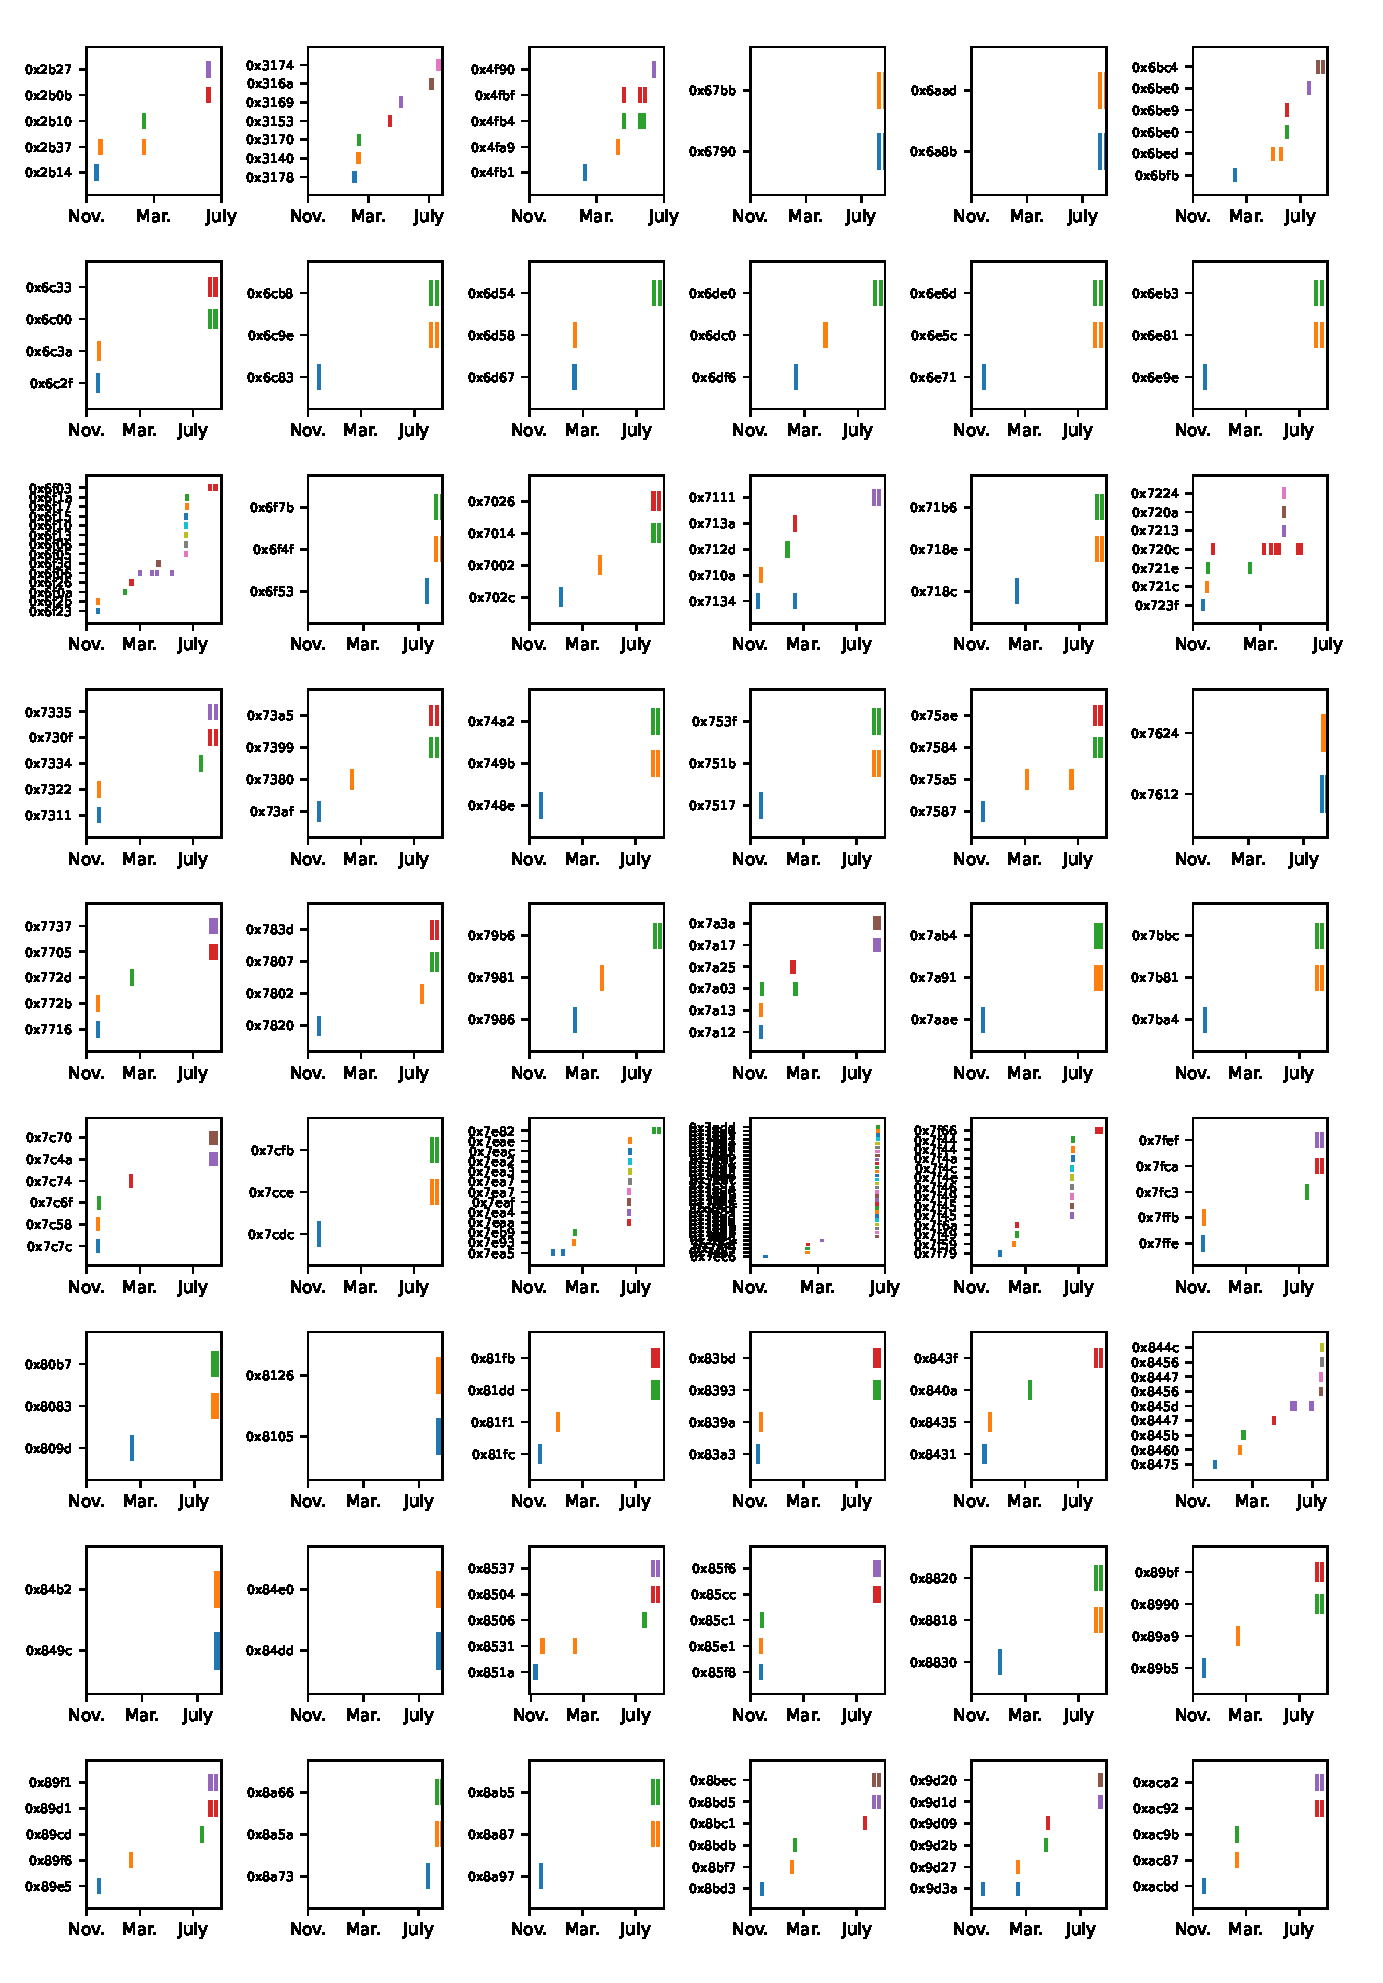
\includegraphics[width=\textwidth]{common/contested.eps}
  \caption{Stake update events in `contested' neighbourhoods}
  \label{event-plot}
\end{figure}

On many of the plots we can observe pairs of addresses that repeatedly top up at very similar times to one another.
%
We reproduce an example listing in Table \ref{event-listing}.
%
\begin{table}
  \centering
  \begin{tabular}{llr}
    \toprule
    Date + time         & Address & Amount (BZZ) \\
    \midrule
    2023-11-21 19:40:00 & 0x6c83 &   11 \\
    2024-07-23 22:15:50 &	0x6c9e  &	10 \\
    2024-07-23 22:16:05 &	0x6cb8  &	10 \\
    2024-08-04 21:56:25 &	0x6c9e  &	10 \\
    2024-08-04 21:56:45 &	0x6cb8  &	10 \\
    \bottomrule
  \end{tabular}
  \caption{Event listing from in bin \code{0x6c8} --- cf.~the eighth plot in Figure \ref{event-plot}}
  \label{event-listing}
\end{table}
%
We posit that the most likely reason for this behaviour is that the same entity started numerous nodes at the same time and placed them in distinct 11-bit neighbourhoods.
%
Since we have sorted by 10-bit neighbourhoods we have caught multiple of these nodes in the same bin, making their activity look like contention.